Para editar los niveles te proponemos un sistema bastante sencillo, el
mismo que hemos utilizado nosotros. Se trata de Tiled, una herramienta libre
y multiplataforma escrita en Java aunque también tienen una versión con Qt.
A continuación os proponemos los pasos para descargarla, instalarla y crear
niveles con ella. ¡Anímate, es muy sencillo!

\subsection{Descargando Tiled}
Para poder usar Tiled necesitas el Java Runtime Enviroment (JRE), la máquina
virtual de Java ya que es el entorno que utiliza. Una vez instalado el JRE
sólo tienes que acudir a su web principal:\\

\href{http://mapeditor.org}{http://mapeditor.org}\\

Aunque también podéis descargarlo directamente a través de este enlace:\\

\href{http://sourceforge.net/projects/tiled/files/Tiled/tiled-0.7.2-bin.zip}{http://sourceforge.net/projects/tiled/files/Tiled/tiled-0.7.2-bin.zip}

\subsection{Utilizando Tiled}

\begin{center}
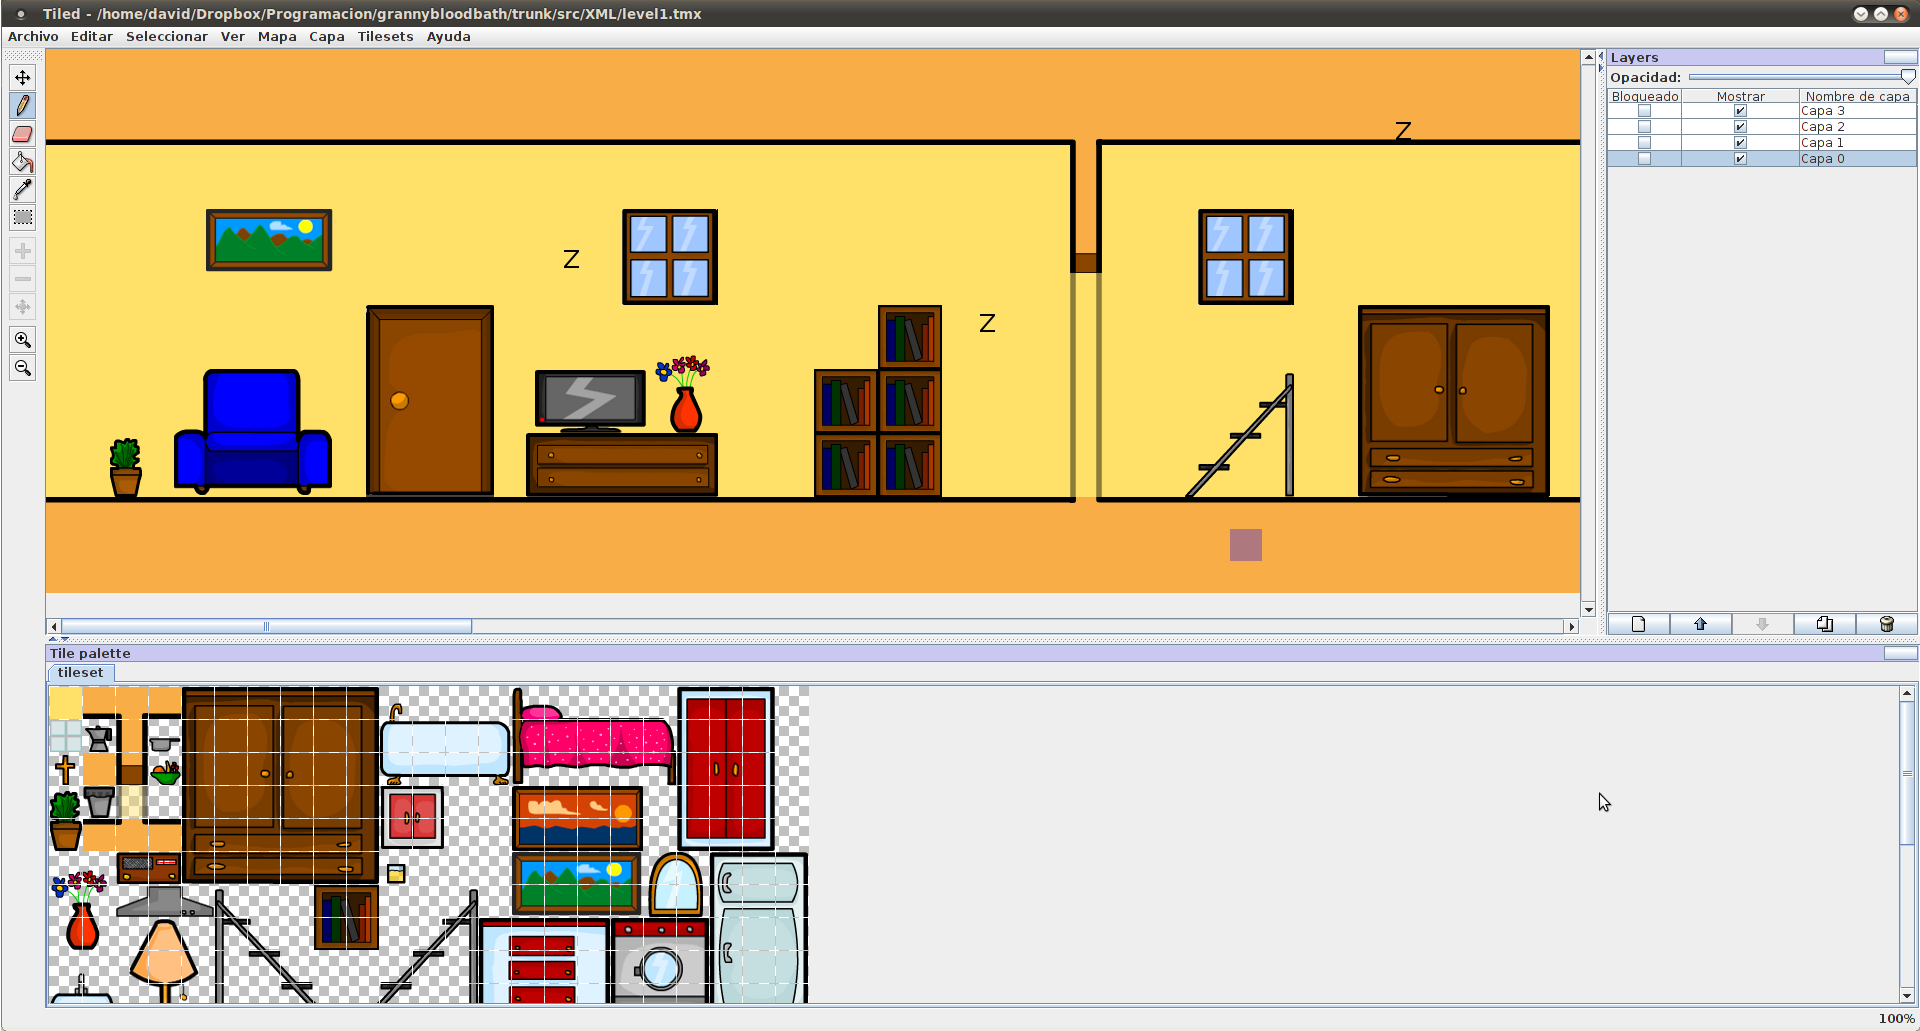
\includegraphics[scale=0.18]{tiled01.png}
\end{center}

Tiled es muy sencillo e intuitivo pero a continuación te explicamos los
elementos básicos de la interfaz para que puedas crear escenarios en un
plis plas:

\begin{itemize}
	\item \emph{Paleta de herramientas}: el panel de la izquierda es
	la barra donde se encuentran las distintas herramientas. Básicamente
	utilizarás el lápic (colocar tiles) y la goma de borrar (eliminar
	tiles).
	\item \emph{Paleta de tiles}: el panel inferior es donde se carga
	el tilset seleccionado. Un tileset es como la paleta de un pintor,
	vas poniendo cuadraditos con la herramienta de lapiz (o tiles) para 
	formar el escenario, como un puzzle. Puedes seleccionar varios
	tiles a la vez arrastrando el raton.
	\item \emph{Barra de capas}: el panel de la derecha es el de las capas
	un escenario de Granny's Bloodbath se compone de 4 capas, las cuales
	explicaremos en el siguiente apartado.	
	\item \emph{Menú}: el típico menú de cualquier aplicación. Desde allí
	podemos cargar niveles, crear nuevos niveles o guardar niveles. También
	podemos cambiar las propiedades y dimensiones del nivel actual.
\end{itemize}

\subsection{Creando escenarios con Tiled desde 0}

El siguiente tutorial explica, paso a paso, cómo hacer un nivel en Tiled para
\emph{Granny's Bloodbath} desde 0. Si quieres ahorrarte complicaciones como
los pasos 2, 3 y 5 puedes elegir un nivel vacío ya configurado en la carpeta
\emph{niveles\_vacios} dentro del directorio del juego.

\begin{enumerate}
	\item Hacemos click en Archivo $\rightarrow$ Nuevo. Nos aparece un diálogo
	y tenemos que seleccionar:
	\begin{itemize}
		\item Tipo de mapa: ortogonal
		\item Tamaño de mapa: anchura la deseada, altura 17 (si
		seleccionamos una altura de tile de 32).
		\item Tamaño de tile: dimensiones de los tiles del tileset
		que utilizaremos. Generalmente $32x32$.
	\end{itemize}
	\item Hacemos click en Tilesets $\rightarrow$ Nuevo tileset. Nos aparece
	un nuevo diálogo que rellenamos de la siguiente manera:
	\begin{itemize}
		\item Nombre del tileset: el deseado
		\item Ancho y alto de tile: como hemos dicho, normalmente
		será 32.
		\item Seleccionamos el checkbox para cargar una imagen y
		pulsamos Navegar para elegirla. Debería estar en el directorio
		multimedia de la carpeta de Granny's Bloodbath.
	\end{itemize}
	\item Creamos las 4 capas necesarias haciendo click sobre el botón
	Añadir capa del panel de capas.
	\begin{itemize}
		\item \emph{Capa 0}: fondo, paredes y objetos que ocupan
		todo el tile.
		\item \emph{Capa 1}: tiles que tienen zonas transparentes,
		se superponen sobre el fondo.
		\item \emph{Capa 2}: tiles que se visualizarán encima de los
		personajes (como si ellos estuvieran por detrás).
		\item \emph{Capa 3}: enemigos y objetos.
	\end{itemize}
	\item Trabajamos rellenando el escenario con los tiles del tileset.
	Presta atención a la capa que tienes seleccionada ya que es posible
	equivocarse. Puedes volver atrás pulsando $Ctrl+Z$.
	\item Ahora debes hacer click en Mapa $\rightarrow$ Propiedades para
	rellenar algunos datos sobre tu nivel:
	\begin{itemize}
		\item tileset\_ancho: número de tiles de ancho del tileset.
		\item tileset\_alto: número de tiles de alto del tileset.
		\item music: código de la música que debe sonar en el nivel.
		Encontrarás los códigos disponibles en el fichero
		XML/resources.xml.
		\item zombie: número de tile del personaje zombie. Normalmente
		viene indicado con una Z. Los números empiezan en 0.
		\item dog: número de tile del perro zombie. Normalmente
		viene indicado con una D. Los números empiezan en 0.
		\item fat: número de tile del zombie gordito. Normalmente
		viene indicado con una F. Los números empiezan en 0.
		\item ammo: número de tile de la munición. Normalmente
		viene indicado con una A. Los números empiezan en 0.
		\item pills: número de tile de las pastillas para la tensión. Normalmente
		viene indicado con una P. Los números empiezan en 0.
		\item teeth: número de tile de la dentadura postiza. Normalmente
		viene indicado con una T. Los números empiezan en 0.
	\end{itemize}
	\item Una vez terminado el mapa hacemos click en Archivo $\rightarrow$
	Guardar como. Elegimos la ruta y el nombre, normalmente deberíamos guardarlo
	en la carpeta XML donde esté situado Granny's Bloodbath.
	\item Para añadir nuestro nuevo nivel al guión tenemos que editar el fichero XML
	XML/plot.xml. Si nuestro nivel se llama `minivel.tmx' el fichero plot.xml
	quedaría de la siguiente manera:\\
	
	\lstinputlisting{plot.xml}
	
	Si nuestro nivel fuera la escena de un enemigo final, en lugar de `level'
	debemos introducir el atributo `boss'.
	
	\item El último paso pasa por editar el fichero del nivel y cambiar la propiedad
	\emph{source} del elemento \emph{image} dentro de \emph{tileset} de:\\
	
	\emph{../multimedia/mi-tileset.png}\\
	
	a:\\
	
	\emph{multimedia/mi-tileset.png}
\end{enumerate}
